\documentclass[tikz,border=10pt]{standalone}
\begin{document}
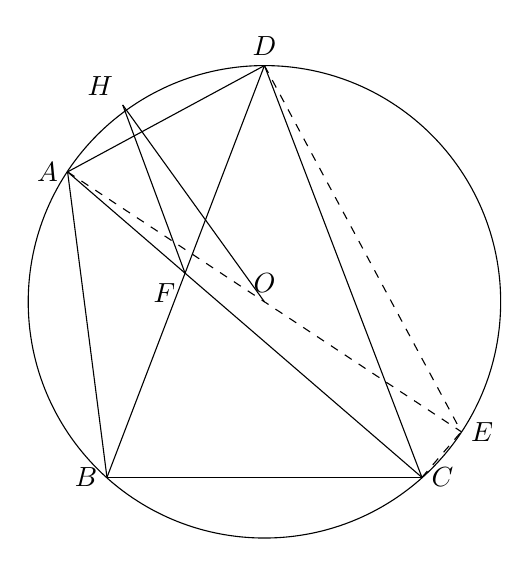
\begin{tikzpicture}
    \coordinate (O) at (0, 0);
    \coordinate (D) at (0, 3);
    \coordinate (A) at (-2.5, 1.65);
    \coordinate (B) at (-2, -2.23);
    \coordinate (C) at (2, -2.23);
    \coordinate (E) at (2.5, -1.65);
    \coordinate (H) at (-1.8, 2.5);
    \coordinate (F) at (-1.007, 0.36);

    \draw (O) circle (3);
    \draw (A) -- (B);
    \draw (B) -- (C);
    \draw (C) -- (D);
    \draw (D) -- (A);
    \draw (A) -- (C);
    \draw (B) -- (D);
    \draw[dashed] (A) -- (E);
    \draw[dashed] (D) -- (E);
    \draw[dashed] (C) -- (E);
    \draw (O) -- (H);
    \draw (H) -- (F);

    \node[left] at (A) {$A$};
    \node[left] at (B) {$B$};
    \node[right] at (C) {$C$};
    \node[above] at (D) {$D$};
    \node[right] at (E) {$E$};
    \node[below left] at (F) {$F$};
    \node[above left] at (H) {$H$};
    \node[above] at (O) {$O$};
\end{tikzpicture}
\end{document}
